%%%%%%%%%%%%%%%%%%%%%%%%%%%%%%%%%%%%%%%%%
% Simple Sectioned Essay Template
% LaTeX Template
%
% This template has been downloaded from:
% http://www.latextemplates.com
%
% Note:
% The \lipsum[#] commands throughout this template generate dummy text
% to fill the template out. These commands should all be removed when 
% writing essay content.
%
%%%%%%%%%%%%%%%%%%%%%%%%%%%%%%%%%%%%%%%%%

%----------------------------------------------------------------------------------------
%	PACKAGES AND OTHER DOCUMENT CONFIGURATIONS
%----------------------------------------------------------------------------------------

\documentclass[12pt]{article} % Default font size is 12pt, it can be changed here

\usepackage{geometry} % Required to change the page size to A4
\geometry{a4paper} % Set the page size to be A4 as opposed to the default US Letter

\usepackage{graphicx} % Required for including pictures

\usepackage{float} % Allows putting an [H] in \begin{figure} to specify the exact location of the figure
\usepackage{wrapfig} % Allows in-line images such as the example fish picture

\usepackage{lipsum} % Used for inserting dummy 'Lorem ipsum' text into the template

\linespread{1.2} % Line spacing

%\setlength\parindent{0pt} % Uncomment to remove all indentation from paragraphs

\graphicspath{{Pictures/}} % Specifies the directory where pictures are stored


\usepackage{amsmath,amsthm}










\newcommand{\e}{\mathrm{e}}



\begin{document}

%----------------------------------------------------------------------------------------
%	TITLE PAGE
%----------------------------------------------------------------------------------------

\begin{titlepage}

\newcommand{\HRule}{\rule{\linewidth}{0.5mm}} % Defines a new command for the horizontal lines, change thickness here

\center % Center everything on the page

\textsc{\LARGE Economics Notes}\\[2cm] % Name of your university/college
%\textsc{\Large Major Heading}\\[0.5cm] % Major heading such as course name
%\textsc{\large Minor Heading}\\[0.5cm] % Minor heading such as course title

\HRule \\[0.8cm]
{ \huge \bfseries Advanced Macroeconomics}\\[0.4cm] % Title of your document
{ \large \bfseries by David Romer}\\[0.1cm]
\HRule \\[1.5cm]

\begin{minipage}{0.4\textwidth}
\begin{flushleft} \large
\emph{}\\
 \textsc{} % Your name
\end{flushleft}
\end{minipage}
~
\begin{minipage}{0.4\textwidth}
\begin{flushright} \large
\emph{Author:} \\
\textsc{Chen} % Supervisor's Name
\end{flushright}
\end{minipage}\\[4cm]
\vfill
{\large \today}\\[2cm] % Date, change the \today to a set date if you want to be precise

%\includegraphics{Logo}\\[1cm] % Include a department/university logo - this will require the graphicx package

 % Fill the rest of the page with whitespace

\end{titlepage}

%----------------------------------------------------------------------------------------
%	TABLE OF CONTENTS
%----------------------------------------------------------------------------------------

\tableofcontents % Include a table of contents

\newpage % Begins the essay on a new page instead of on the same page as the table of contents 

%----------------------------------------------------------------------------------------
%	INTRODUCTION
%----------------------------------------------------------------------------------------

\section{Solow Growth Model} % Major section

%Example citation \cite{Figueredo:2009dg}.

%------------------------------------------------

\subsection{Setup} % Sub-section
Given the assumption of constant returns to scale, the production function is $Y(t)=F(K(t),A(t)L(t))$ or alternatively in intensive form $y(t)=f(k(t))$ in which $y=Y/(AL)$ and $k=K/(AL)$. $f(k)$ is assumed to satisfy $f(0)=0,f'(k)>0,f"(0)<0$ and the Inada conditions: $\lim_{k\rightarrow 0}f'(k)=\infty,\lim_{k\rightarrow \infty}f'(k)=0$. The evolution of the inputs into production are determined by
\begin{align*}
	\dot{L}(t) & =nL(t), \\
	\dot{A}(t) & =gA(t), \\
	\dot{K}(t) & =sY(t)-\delta K(t).
\end{align*}
These equations yield solution as follows
\begin{align*}
L(t) & =L(0)\e^{nt} \\
A(t) & =A(0)\e^{gt} .
\end{align*}
Labor and knowledge grow at constant rates $n$ and $g$ respectively. Since the production function $F(K,AL)$ is not specified, we cannot give an explicit solution of $K(t)$. 

\subsection{Stable Solution} % Sub-section
For the sake of qualitative analysis, the system of differential equations can be simplified to a single differential equation with respect to $k(t)$:
\[
\dot{k}(t)=sf(k)-(n+g+\delta)k(t).
\]
\begin{figure}[H] % Example image
	\center{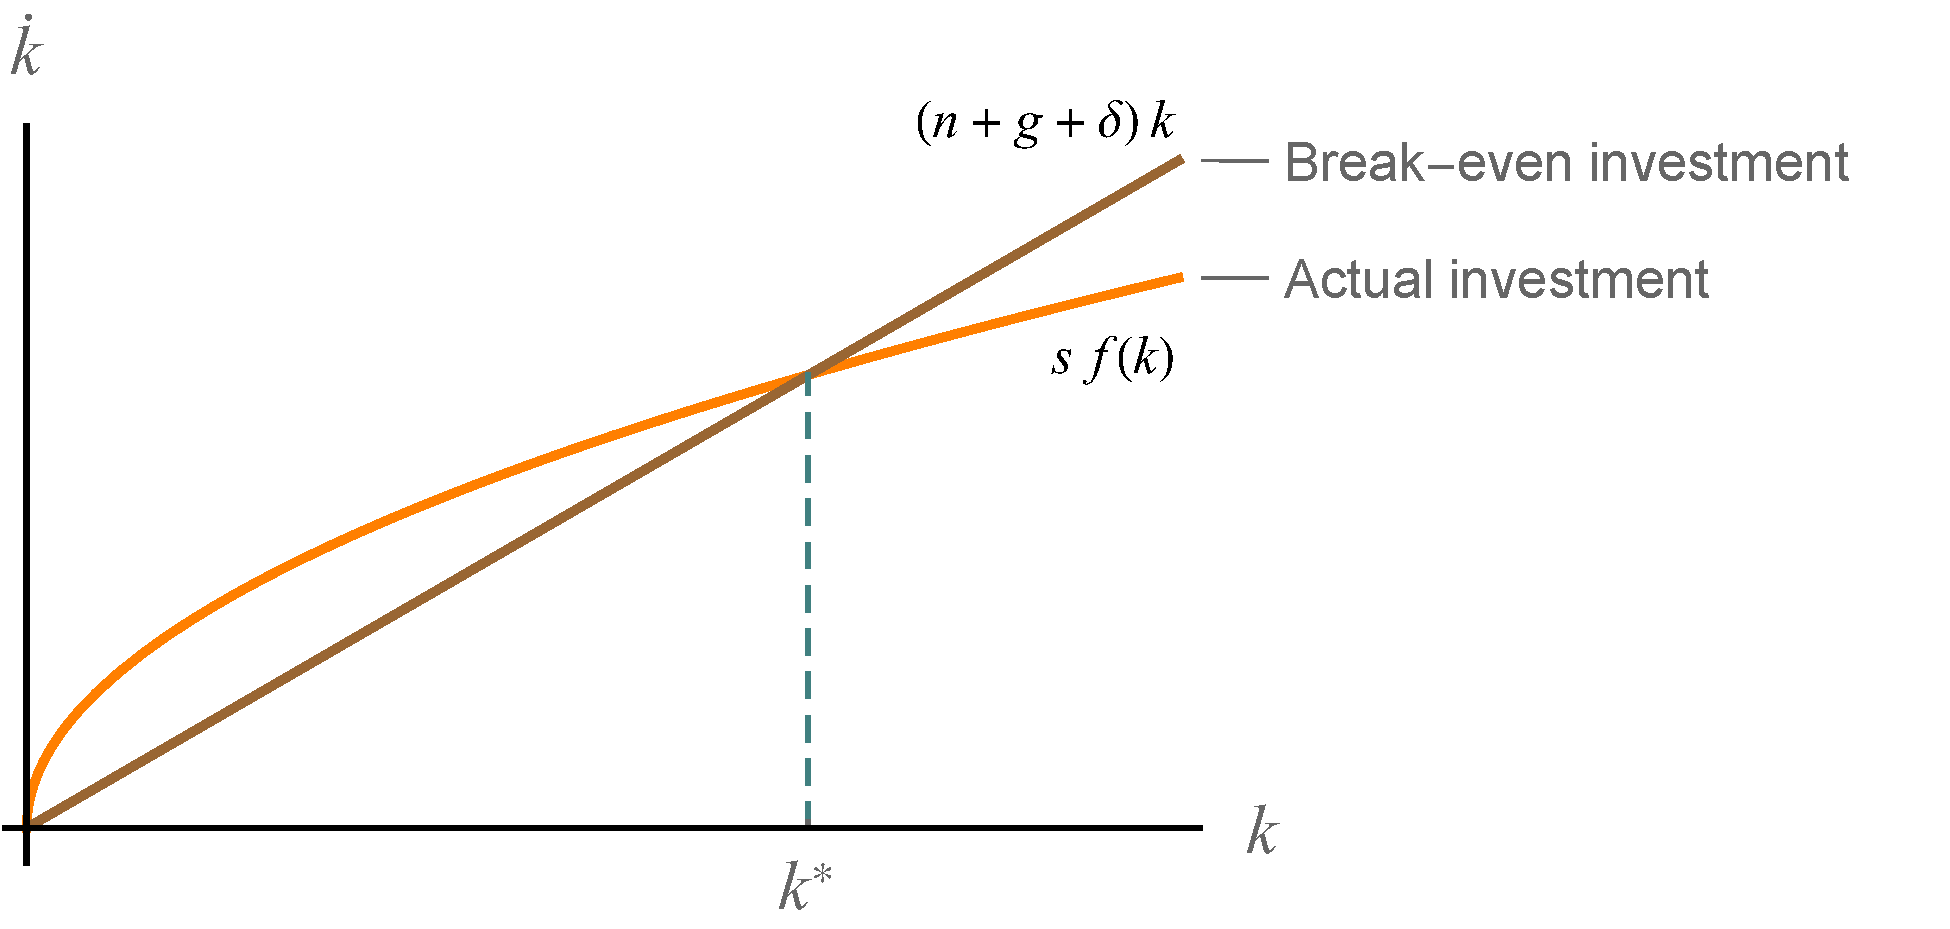
\includegraphics[width=0.85\linewidth]{fig1}}
	\caption{Actual and break-even investment}
	\label{fig:speciation}
\end{figure}
As the figure illustrates, the equation $sf(k)-(n+g+\delta)k(t)=0$ has unique solution $k^*=k^*(s,n,g,\delta)$. Then we can readily employ the diagrammatic analysis to find the stable solution. It is clear to see that regardless of where $k$ starts, it converge to $k^*$ and remains there.
\begin{figure}[H] % Example image
	\center{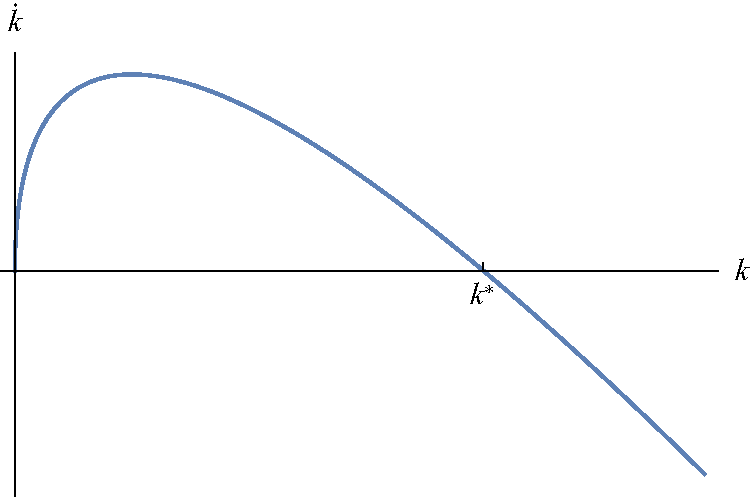
\includegraphics[width=0.6\linewidth]{fig2}}
	\caption{\small Phase diagram for $k$}
	\label{fig:speciation}
\end{figure}
When $t\rightarrow\infty$, the economy reaches its balanced growth path and thus we see
\begin{align*}
k(t) & \rightarrow k^*\\
y(t) & \rightarrow f(k^*)\\
L(t) & =L(0)\e^{nt} \\
A(t) & =A(0)\e^{gt} \\
K(t) & \sim K(0)\e^{(n+g)t}\\
Y(t) & \sim Y(0)\e^{(n+g)t}.
\end{align*}

\subsection{Consumption}
While $s$ of the production $Y(t)$ are invested for more consumption in the future, the current consumption $C(t)$ accounts for $1-s$ of the production $Y(t)$. Let $c(t)$ denote the consumption per unit of effective labor, that  is
\[
c(t)=(1-s)f(k).
\]
On the balanced growth path it follows that
\[
c^*=(1-s)f(k^*)=f(k^*)-(n+g+\delta)k^*.
\] 

\subsection{The Impact of a Change in Saving Rate}
\subsubsection{The Impact on Output}
\begin{figure}[H] % Example image
	\center{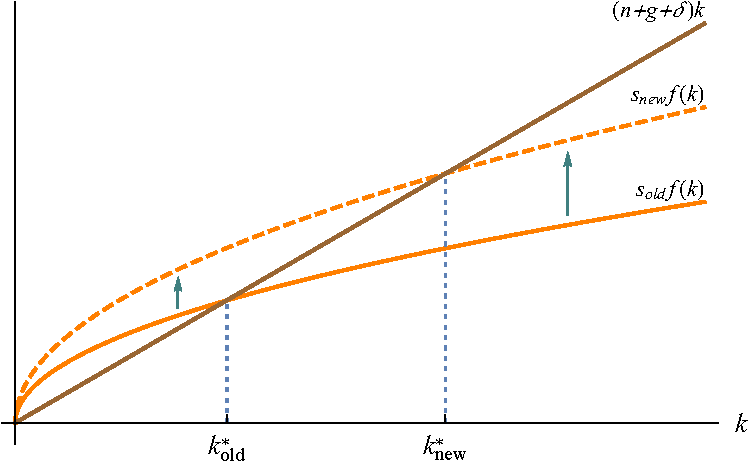
\includegraphics[width=0.75\linewidth]{fig3}}
	\caption{\small The effects of an increase in saving rate on investment}
	\label{fig:speciation}
\end{figure}

\begin{figure}[H] % Example image
	\center{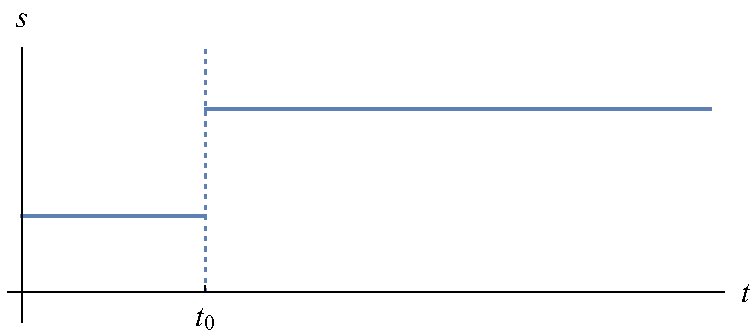
\includegraphics[width=0.55\linewidth]{fig4_1}}
	\center{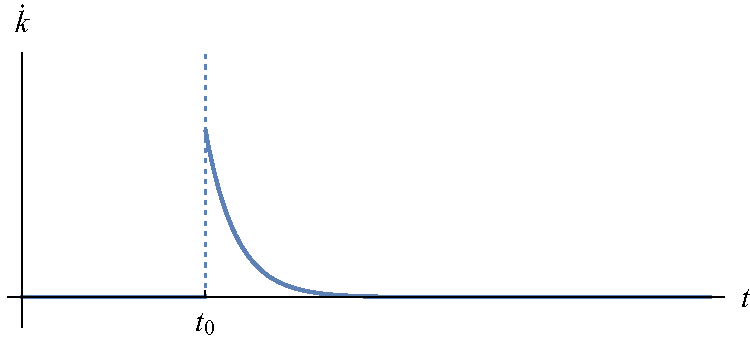
\includegraphics[width=0.55\linewidth]{fig4_2}}
	\center{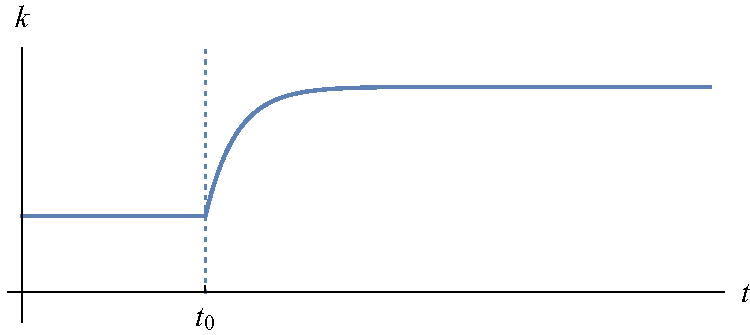
\includegraphics[width=0.55\linewidth]{fig4_3}}
	\center{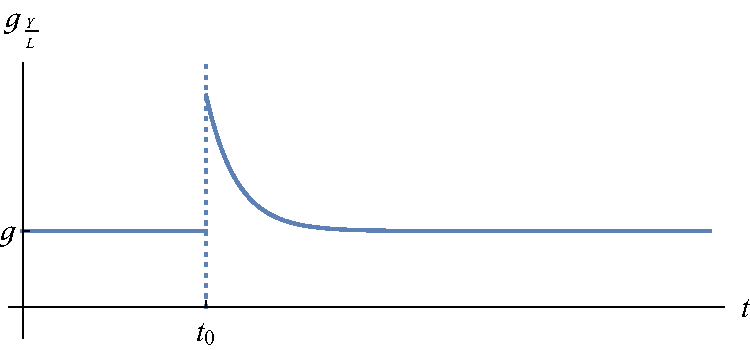
\includegraphics[width=0.55\linewidth]{fig4_4}}
	\center{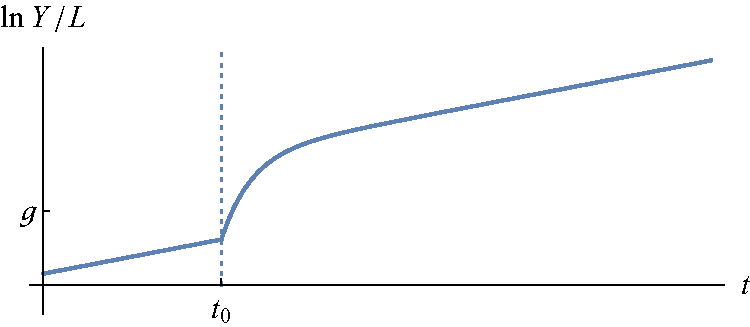
\includegraphics[width=0.55\linewidth]{fig4_5}}
	\caption{\small The effects of an increase in saving rate}
	\label{fig:speciation}
\end{figure}

\subsubsection{The Impact on Consumption}

\begin{figure}[H] % Example image
	\center{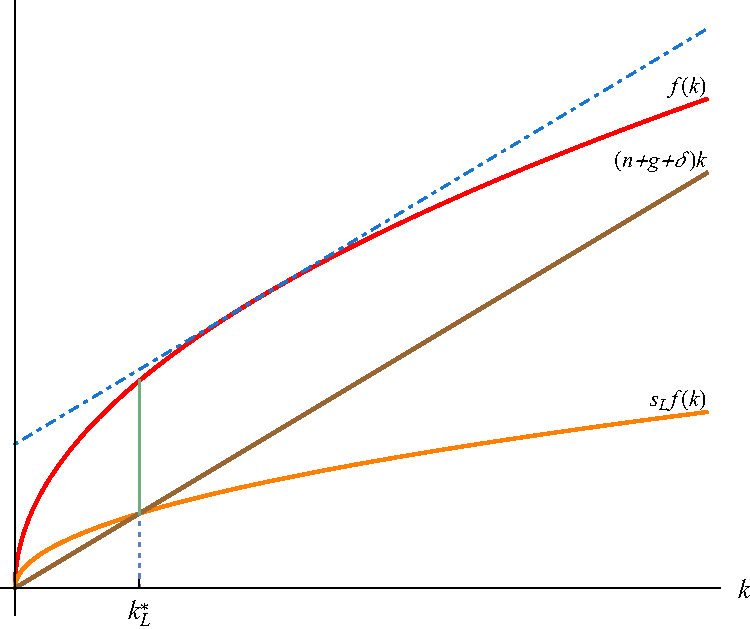
\includegraphics[width=0.5\linewidth]{fig5_1}}
	\center{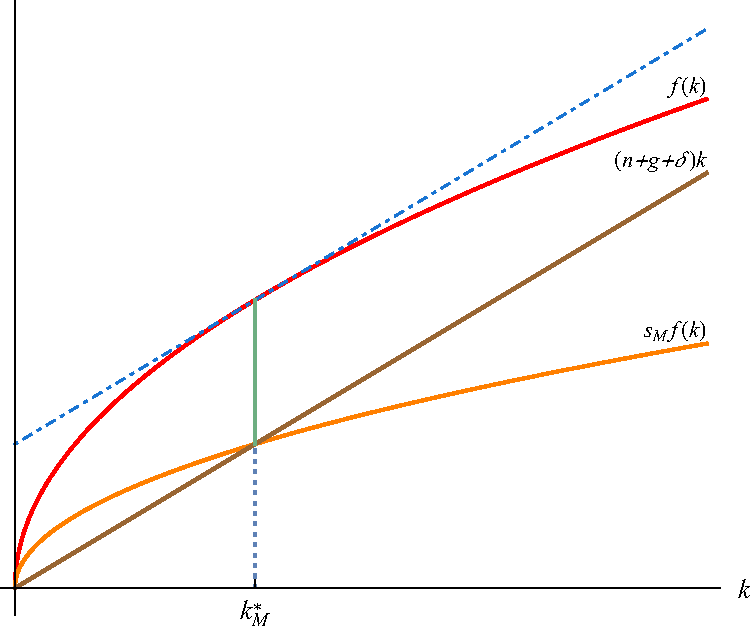
\includegraphics[width=0.5\linewidth]{fig5_2}}
	\center{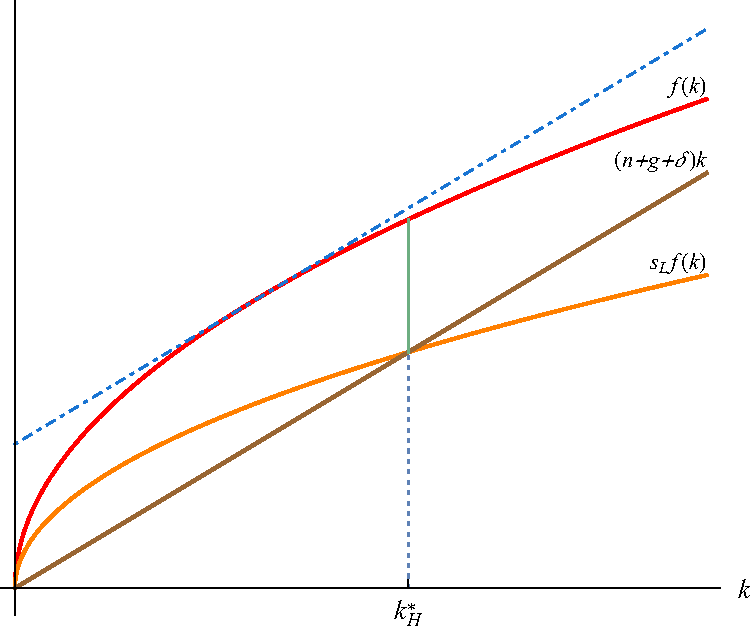
\includegraphics[width=0.5\linewidth]{fig5_3}}
	\caption{\small The effects of an increase in saving rate on consumption}
	\label{fig:speciation}
\end{figure}


\begin{figure}[H] % Example image
	\center{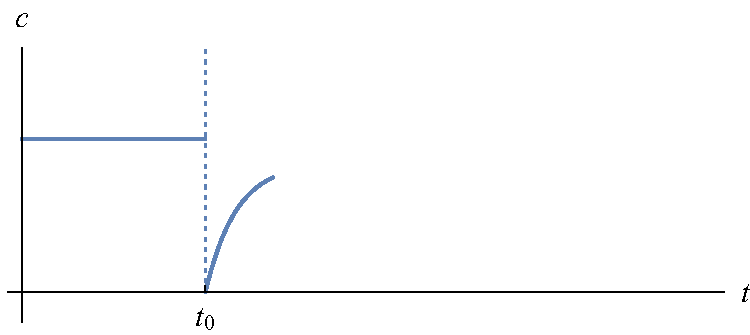
\includegraphics[width=0.55\linewidth]{fig6}}
	\caption{\small The effects of an increase in saving rate on consumption}
	\label{fig:speciation}
\end{figure}


\subsection{Typical Example}

Setting $Y=K^\alpha (AL)^{1-\alpha}\;(0<\alpha<1)$ and accordingly $y(t)=k(t)^\alpha$, we get the differential equation with respect to $k(t)$:
\[
\dot{k}=sk^\alpha-(n+g+\delta)k.
\]
The capital per unit of effective labor 
\[
k(t)=\left[\dfrac{\widetilde{C}\e^{-(1-\alpha)(n+g+\delta)t}+s}{n+g+\delta}\right]^{\tfrac{1}{1-\alpha}}.
\]
solves the equation, where $\widetilde{C}$ is a constant to be specified by the initial condition $k(0)=k_0$. On the balanced growth path, 
\[
\lim\limits_{t\rightarrow+\infty}k(t)=k^*=\left(\dfrac{s}{n+g+\delta}\right)^{1/(1-\alpha)}
\]
%------------------------------------------------

\subsection{Quantitative Implications}
Since $y^*(s,n,g,\delta)=f(k^*(s,n,g,\delta))$,
\[
\frac{\partial y^*}{\partial s}=\frac{\partial k^*}{\partial s}f'(k^*)
\]
\[
\frac{\partial k^*}{\partial s}=\frac{f(k^*)}{(n+g+\delta)-sf'(k^*)}
\]
\begin{align*}
\frac{s}{y^*}\frac{\partial y^*}{\partial s}&=\frac{s}{y^*}\frac{f'(k^*)f(k^*)}{(n+g+\delta)-sf'(k^*)}\\
&=\frac{\alpha_K(k^*)}{1-\alpha_K(k^*)}
\end{align*}

\newpage


\section{The Ramsey-Cass-Koopmans Model} 
\subsection{Setup} % Sub-section
Households' maximization problem is 
\[
\max\; B\int_{0}^{\infty}e^{-\beta t}\frac{c(t)^{1-\theta}}{1-\theta}dt
\]
\[
\mathrm{s.t.}\;k'(t)=f(k(t))+c(t)-(n+g)k(t) 
\]
where $B=A(0)^{1-\theta}L(0)/H$, $\beta=\rho-n-(1-\theta)g$. Hamilton function is
\[
H=e^{-\beta t}\frac{c(t)^{1-\theta}}{1-\theta}+\lambda(t)[f(k(t))+c(t)-(n+g)k(t)],
\]
which leads to Hamilton equations
\begin{align*}
\frac{\partial H}{\partial c} & =e^{-\beta t}c^{-\theta}+\lambda=0,\\
\frac{\partial H}{\partial k} & =\lambda [f'(k)-(n+g)]=-\lambda'.
\end{align*}
Substituting $\beta$ into it yields the Euler equation
\[
\frac{c'}{c}=\frac{f'(k)-\rho-\theta g}{\theta}
\]



\subsection{Stable Solution} 



\begin{figure}[H] % Example image
	\center{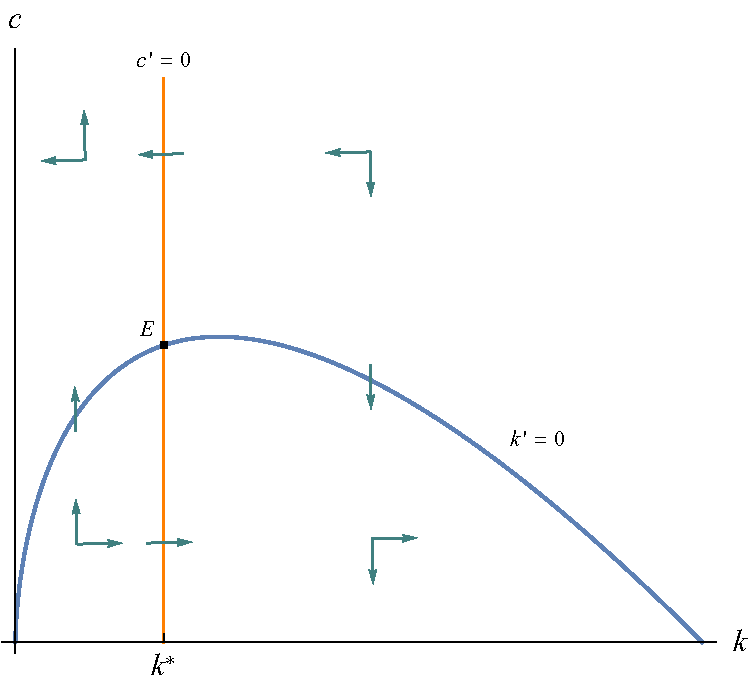
\includegraphics[width=0.8\linewidth]{fig7}}
	\caption{\small The dynamics of $k$ and $c$}
	\label{fig:speciation}
\end{figure}

\section{The Diamond Model}
\subsection{Setup} % Sub-section
Let $C_{1,t}$ and $C_{2,t+1}$ denote the consumption in period $t$ of young and old individuals.
Households' maximization problem is 
\[
\max\; \frac{C_{1,t}^{1-\theta}}{1-\theta}+\frac{1}{1+\rho}\frac{C_{2,t+1}^{1-\theta}}{1-\theta}
\]
\[
\mathrm{s.t.}\;C_{1,t}+ \frac{1}{1+r_{t+1}}C_{2,t+1}=A_tw_t
\]
The Euler equation is 
\[
\frac{C_{2,t+1}}{C_{1,t}}=\left(\frac{1+r_{t+1}}{1+\rho}\right)^{\tfrac{1}{\theta}}
\]

\section{Content Section} % Major section

\lipsum[5] % Dummy text

%------------------------------------------------

\subsection{Subsection 1} % Sub-section

\subsubsection{Subsubsection 1} % Sub-sub-section

\lipsum[6] % Dummy text

%------------------------------------------------

\subsubsection{Subsubsection 2} % Sub-sub-section

\lipsum[6] % Dummy text
%\begin{wrapfigure}{l}{0.4\textwidth} % Inline image example
%  \begin{center}
%    \includegraphics[width=0.38\textwidth]{fish}
%  \end{center}
%  \caption{Fish}
%\end{wrapfigure}
\lipsum[7-8] % Dummy text

%------------------------------------------------

\subsubsection{Subsubsection 3} % Sub-sub-section

\begin{description} % Numbered list example

\item[First] \hfill \\
\lipsum[9] % Dummy text

\item[Second] \hfill \\
\lipsum[10] % Dummy text

\item[Third] \hfill \\
\lipsum[11] % Dummy text

\end{description} 

%----------------------------------------------------------------------------------------
%	MAJOR SECTION X - TEMPLATE - UNCOMMENT AND FILL IN
%----------------------------------------------------------------------------------------

%\section{Content Section}

%\subsection{Subsection 1} % Sub-section

% Content

%------------------------------------------------

%\subsection{Subsection 2} % Sub-section

% Content

%----------------------------------------------------------------------------------------
%	CONCLUSION
%----------------------------------------------------------------------------------------

\section{Conclusion} % Major section

\lipsum[12-13]

%----------------------------------------------------------------------------------------
%	BIBLIOGRAPHY
%----------------------------------------------------------------------------------------

\begin{thebibliography}{99} % Bibliography - this is intentionally simple in this template

\bibitem[Figueredo and Wolf, 2009]{Figueredo:2009dg}
Figueredo, A.~J. and Wolf, P. S.~A. (2009).
\newblock Assortative pairing and life history strategy - a cross-cultural
  study.
\newblock {\em Human Nature}, 20:317--330.
 
\end{thebibliography}

%----------------------------------------------------------------------------------------

\end{document}